%%%%%%%%%%%%%%%%%%%%%%%%%%%%%%%%%%%%%%%%%%%%%%%%%%%%%%%%%%%%%%%%%%%%%%%%%%%%%%%%
\subsection{Πειραματική διάταξη}
\label{subsection:02_05_03:01}

Η πειραματική διαδικασία διεξάγεται με τη χρήση των ίδιων πέντε συνόλων
δεδομένων αναφοράς $D = \{D_k\}$, $k \in \{0,1,\dots,4\}$ τα οποία
χρησιμοποιήθηκαν στο προηγούμενο κεφάλαιο για τη δοκιμή και εξακρίβωση της
επίδοσης των αλγορίθμων που κατασκευάσαμε και των αλγορίθμων της βιβλιογραφίας
(Πίνακας \ref{tbl:02:04_05:dataset_sizes}).

Η πειραματική διάταξη είναι η ακόλουθη. Οι ακτίνες κάθε δείγματος του συνόλου
δεδομένων $D_k^d$, $k \in \{0,1,\dots,4\}$, $d \in \{0,1,\dots,|D_k|\}$ πρώτα
προβάλλονται στο επίπεδο $x-y$ γύρω από τη στάση $\bm{r}_k^d$. Οι σαρώσεις των
συνόλων δεδομένων δεν είναι πανοραμικές, επομένως ο υπόλοιπος γωνιακός χώρος
συμπληρώνεται με ένα ημικυκλικό τόξο που ενώνει τις δύο ακραίες ακτίνες της
κάθε σάρωσης. Η ακτίνα του ημικυκλίου ορίζεται ως η ελάχιστη των δύο ακραίων
ακτίνων του $D_k^d$. Διαφορετικοί τρόποι για το κλείσιμο του περιβάλλοντος
(π.χ.  μέσω καθρεφτισμού των μετρήσεων κατά $x$ ή $y$, ή ένωσης των δύο ακραίων
ακτίνων μέσω ευθύγραμμου τμήματος) έχουν βρεθεί ισοδύναμοι όσον αφορά στην
επίδοση των υπό δοκιμής μεθόδων. Το σύνολο σημείων που προκύπτει θεωρείται ως ο
περιβάλλον χώρος $\bm{W}_k^d$ του αισθητήρα αποστάσεων. Η πρώτη πραγματική
στάση του αισθητήρα $\bm{p}_{0,k}^d$ παράγεται τυχαία εντός του πολυγώνου που
σχηματίζεται από το σύνολο σημείων $\bm{W}_k^d$. Η σάρωση $\mathcal{S}_{0,k}^d$
υπολογίζεται μέσω δεσμοβολής $N_s$ ακτίνων από τη στάση $\bm{p}_{0,k}^d$ προς
τις ακμές του πολυγώνου που σχηματίζεται από τα σημεία του συνόλου
$\bm{W}_k^d$, σε ένα γωνιακό πεδίο όρασης $\lambda = 2\pi$. Η δεύτερη στάση του
αισθητήρα $\bm{p}_{1,k}^d$ λαμβάνεται μέσω διαταραχής των συνιστωσών της στάσης
$\bm{p}^d_{0,k}$ με ποσότητες που εξάγονται από ομοιόμορφες κατανομές σφαλμάτων
$U_{xy}(-\overline{\delta}_{xy}, \overline{\delta}_{xy})$,
$U_{\theta}(-\overline{\delta}_{\theta}, \overline{\delta}_{\theta})$:
$\overline{\delta}_{xy}$, $\overline{\delta}_\theta$ $\in \mathbb{R}_{\geq 0}$.
Η σάρωση $\mathcal{S}_{1,k}^d$ υπολογίζεται ομοίως μέσω δεσμοβολής $N_s$
ακτίνων από τη στάση $\bm{p}_{1,k}^d$ προς τις ακμές του $\bm{W}_k^d$, σε ένα
γωνιακό πεδίο όρασης $\lambda = 2\pi$.  Για την αξιολόγηση της επίδοσης των
αλγορίθμων υπό δοκιμή ως προς τις αρχικές συνθήκες μετατόπισης συμμορφωνόμαστε
με, και υιοθετούμε, την πειραματική διάταξη του Censi \cite{Censi2008a}, η
οποία συνίσταται στην προοδευτική αύξηση της απόστασης μεταξύ των συνιστωσών
των δύο στάσεων. Οι εν λόγω διαμορφώσεις παρατίθενται στον πίνακα
\ref{tbl:02:05_03:deltas}.


Προκειμένου να ελεγχθεί η επίδοση των αλγορίθμων σε πραγματικές συνθήκες
δοκιμάζονται πέντε επίπεδα θορύβου με επίδραση στις μετρήσεις των σαρώσεων
$\mathcal{S}_{0,k}^d$, $\mathcal{S}_{1,k}^d$: κάθε μέτρηση διαταράσσεται από
θόρυβο $\mathcal{N}_R \sim (0, \sigma_R^2)$: $\sigma_R \in \{0.01, 0.03,
0.05, 0.10, 0.20\}$ m. Οι τιμές των τυπικών αποκλίσεων υπολογίστηκαν από
εμπορικά διαθέσιμους πανοραμικούς αισθητήρες lidar, προσδιορίζοντας το μέγεθος
της μέγιστης αναφερόμενης τιμής των σφαλμάτων απόστασης τους και διαιρώντας το
με τον συντελεστή τρία. Το σκεπτικό είναι ότι $99.73\%$ των σφαλμάτων
εντοπίζονται εντός $3\sigma$ γύρω από την πραγματική απόσταση μεταξύ μιας
ακτίνας και ενός εμποδίου, υποθέτοντας ότι τα σφάλματα κατανέμονται κανονικά. Η
ελάχιστη τιμή $\sigma_R = 0.01$ m αναφέρεται για ακριβείς πανοραμικούς
αισθητήρες μεγάλου κόστους VELODYNE \cite{velodyne_datasheet}, και οι υπόλοιπες
για πανοραμικούς αισθητήρες με ελκυστική τιμή, αλλά αυξημένα επίπεδα
διαταραχών, π.χ. RPLIDAR A2M8, YDLIDAR G4, G6, TG30 και X4
\cite{a2m8_datasheet,ydlidar}. Το μέγεθος των σαρώσεων εισόδου ορίστηκε σε
$N_s=360$ ακτίνες.
\begin{table}\centering
  \begin{tabular}{ll}
  Συντομογραφία         & Διαμόρφωση (m,rad)                                                      \\  \toprule
  $\Delta_0$            & $(\overline{\delta}_{xy}, \overline{\delta}_{\theta}) = (0.05, 0.035)$  \\
  $\Delta_1$            & $(\overline{\delta}_{xy}, \overline{\delta}_{\theta}) = (0.10, 0.070)$  \\
  $\Delta_2$            & $(\overline{\delta}_{xy}, \overline{\delta}_{\theta}) = (0.15, 0.150)$  \\
  $\Delta_3$            & $(\overline{\delta}_{xy}, \overline{\delta}_{\theta}) = (0.20, 0.300)$  \\
  $\Delta_4$            & $(\overline{\delta}_{xy}, \overline{\delta}_{\theta}) = (0.20, 0.560)$  \\
  $\Delta_5$            & $(\overline{\delta}_{xy}, \overline{\delta}_{\theta}) = (0.20, \pi/4)$  \\  \bottomrule
  \end{tabular}
\caption{\small Οι διαμορφώσεις των μέγιστων αποστάσεων μεταξύ οποιωνδήποτε δύο
         στάσεων του αισθητήρα με βάση τις οποίες δοκιμάσθηκε η απόκριση όλων
         των μεθόδων. Οι δύο στάσεις έχουν απόσταση κατά συνιστώσα θέσης
         $U_{xy}(-\overline{\delta}_{xy}, \overline{\delta}_{xy})$, και
         κατά προσανατολισμό
         $U_{\theta}(-\overline{\delta}_{\theta}, \overline{\delta}_{\theta})$,
         όπου με $U(\alpha,\beta)$ συμβολίζεται η ομοιόμορφη συνεχής κατανομή}
  \label{tbl:02:05_03:deltas}
\end{table}

Ο ελάχιστος και ο μέγιστος ρυθμός υπερδειγματοληψίας του χάρτη για τη μέθοδο
\texttt{fsm} ορίστηκε σε $(\mu_{\min},\mu_{\max}) \equiv
(2^{\nu_{\min}},2^{\nu_{\max}}) \equiv (2^0,2^3)$, και ο αριθμός των
επαναλήψεων της συνιστώσας εκτίμησης θέσης ορίστηκε σε $I_T=5\nu$, $\nu \in
\mathbb{Z}_{\geq 0}: \nu \in [\nu_{\min}, \nu_{\max}]$. Το κριτήριο σύγκλισης
για όλες τις μεθόδους εφαρμόσθηκε μόνο ως προς την διαφορά εκτίμησης του
προσανατολισμού: $\varepsilon_{\delta p} = 10^{-5}$. Σε αντίθεση με τον FSMSM ο
FSM δεν υιοθετεί κριτήριο τερματισμού (Αλγόριθμος
\ref{alg:algorithm_fsmsm}:\ref{alg:fsmsm_termination_criterion_start}-\ref{alg:fsmsm_termination_criterion_end})
για λόγους εξοικονόμησης χρόνου εκτέλεσης. Για τον ίδιο λόγο τέθηκε άνω όριο
στον αριθμό επανεκκινήσεων λόγω μετατόπισης της εκτίμησης θέσης εκτός του χάρτη
$\widetilde{\bm{M}}$, με τιμή $R_{\max} = 100$ επανεκκινήσεις.

Για σκοπούς σύγκρισης της επίδοσης του FSM με μεθόδους ευθυγράμμισης σαρώσεων η
πειραματική διαδικασία διενεργείται έναντι των μεθόδων ευθυγράμμισης
Μετασχηματισμού Κανονικών Κατανομών (Normal Distributions Transform---NDT)
\cite{Bibera,ndt_code}, FastGICP \cite{Segal2009a,fgicp_code}, και PLICP
\cite{Censi2008a,plicp_code}. Οι NDT, FastGICP και PLICP ανήκουν στις
\textit{καθιερωμένες} μεθόδους ευθυγράμμισης σαρώσεων
\cite{Koide2021a,Xu2018b,Sobreira2019b,Pishehvari2019b,Qingshan2019c,Pham2021b}.
Επιπλέον, για λόγους σύγκρισης έναντι σύγχρονων αλγορίθμων, οι πειραματική
διαδικασία επεκτείνεται στους αλγορίθμους FastVGICP
\cite{Koide2021a,fgicp_code} και NDT-PSO \cite{Bouraine2021,ndt_pso_code}. Η
πειραματική διαδικασία δεν περιλαμβάνει αυτή τη φορά τη μέθοδο TEASER λόγω της
αδυναμίας εκτέλεσής της σε χρόνους τέτοιους που να συμβαδίζουν με το ρυθμό
ανανέωσης μετρήσεων από έναν τυπικό αισθητήρα lidar.

Για κάθε πείραμα οι μέθοδοι PLICP, NDT, FastGICP, FastVGICP, NDT-PSO, και
\texttt{fsm} εκτελέσθηκαν για $E = 10$ φορές για όλα τα δείγματα των $D_k \in D
\equiv \{$\texttt{aces}, \texttt{fr079}, \texttt{intel}, \texttt{mit\_csail},
\texttt{mit\_killian}$\}$, $k \in \{0,1,\dots,4\}$, για κάθε διαμόρφωση
μέγιστων αποστάσεων στάσεων (πίνακας \ref{tbl:02:05_03:deltas}), και κάθε
επίπεδο θορύβου $\sigma_R$.  Επομένως κάθε μέθοδος δοκιμάστηκε συνολικά
$N_{tot} = 10 \times 6 \times 5 \times \sum |D_k|\approx
1.36$$\cdot10$$\texttt{e}$$+$$7$ φορές.

Για κάθε τελική εκτίμηση στάσης $\hat{\bm{p}}_{1,k,e}^{\prime d}$ που εξάγεται
από κάθε αλγόριθμο, $d = 1,2,\dots,|D_k|$, $k \in \{0,1,\dots,4\}$,
$e=1,2,\dots,E$, καταγράφεται η απόκλισή της από την πραγματική στάση
$\bm{p}_{1,k,e}^d$ με τη μορφή του μέτρου σφάλματος θέσης και προσανατολισμού

Τα πειράματα επί των FSM, FastGICP, FastVGICP, PLICP, και NDT πραγματοποιήθηκαν
σε ένα μόνο νήμα, σε υπολογιστή με συχνότητα CPU $4.0$ GHz. Ο NDT-PSO είναι
παράλληλη υλοποίηση: τα πειράματά του διεξήχθησαν σε τέσσερα νήματα, σε
υπολογιστή με συχνότητα CPU $2.2$ GHz.




%%%%%%%%%%%%%%%%%%%%%%%%%%%%%%%%%%%%%%%%%%%%%%%%%%%%%%%%%%%%%%%%%%%%%%%%%%%%%%%%
\subsection{Αποτελέσματα}
\label{subsection:02_05_03:02}

Τα σχήματα \ref{fig:02_05_03:02:01} και \ref{fig:02_05_03:02:02} παρουσιάζουν
τις κατανομές σφαλμάτων θέσης και προσανατολισμού αντίστοιχα, για κάθε
αλγόριθμο, επίπεδο διαταραχών που επιδρούν στις μετρήσεις του αισθητήρα, και
διαμόρφωση αρχικών συνθηκών $\Delta_\ast$ (πίνακας \ref{tbl:02:05_03:deltas}),
κατά μήκός όλων των εκτιμήσεων στάσης που προέκυψαν μέσω της πειραματικής
διαδικασίας. Το σχήμα \ref{fig:02_05_03:02:03} παρουσιάζει τις κατανομές των
χρόνων εκτέλεσης για τις ίδιες διατάξεις. Τα σχήματα \ref{fig:02_05_03:02:04}
και \ref{fig:02_05_03:02:05} παρουσιάζουν τη σχέση ανάμεσα στις αρχικές
συνθήκες μετατόπισης και τις τελικές συνθήκες σφαλμάτων για τη συνιστώσα της
θέσης και τη συνιστώσα του προσανατολισμού αντίστοιχα, για τη διαμόρφωση όπου
$(\overline{\delta}_{xy}, \overline{\delta}_{\theta}) = (0.20, \pi/4)$ [m,rad],
για κάθε επίπεδο διαταραχών που επιδρούν στις μετρήσεις του αισθητήρα.  Τα
σχήματα \ref{fig:appendix_05_01:01}-\ref{fig:appendix_05_01:12} απεικονίζουν
την ίδια σχέση για όλες τις υπό δοκιμή διαμορφώσεις $\Delta_\ast$.  Τα σχήματα
\ref{fig:02_05_03:02:06} και \ref{fig:02_05_03:02:07} απεικονίζουν την ίδια
σχέση, αλλά με εστίαση στο κάτω όριο σφαλμάτων, με άνω όριο τον μέσο όρο
σφάλματος όλων των μεθόδων για τη διαμόρφωση όπου $(\overline{\delta}_{xy},
\overline{\delta}_{\theta}) = (0.20, \pi/4)$ [m,rad]. Τα σχήματα
\ref{fig:appendix_05_01:13}-\ref{fig:appendix_05_01:24} απεικονίζουν την ίδια
συνθήκη για όλες τις υπό δοκιμή διαμορφώσεις $\Delta_*$. Το σχήμα
\ref{fig:02_05_03:02:08} απεικονίζει τον αριθμό των επανεκκινήσεων της μεθόδου
\texttt{fsm} συναρτήσει των αρχικών συνθηκών μετατόπισης για όλα τα
δοκιμασθέντα επίπεδα διαταραχών μέτρησης και όλες τις διαμορφώσεις αρχικών
συνθηκών μέγιστης μετατόπισης.

\begin{figure}\vspace{1cm}\hspace{0.5cm}
  \input{./figures/parts/02/chapters/05/sections/03/position_errors.tex}
  \vspace{-4cm}
  \caption{\small Οι κατανομές των σφαλμάτων εκτίμησης θέσης για κάθε αλγόριθμο
           με βάση την πειραματική διάταξη της ενότητας
           \ref{subsection:02_05_03:01}. Κάθε ορθογώνιο αντιπροσωπεύει τα
           στατιστικά $\approx 4.5$$\cdot$$10$\texttt{e}$+$$5$ ευθυγραμμίσεων.
           Οι κουκκίδες αντιπροσωπεύουν ολικά μέσα σφάλματα εκτίμησης}
  \label{fig:02_05_03:02:01}
\end{figure}


\begin{figure}\vspace{1cm}\hspace{0.5cm}
  \definecolor{c1}{rgb}{0 0.4470 0.7410}
\definecolor{c2}{rgb}{0.8500 0.3250 0.0980}
\definecolor{c3}{rgb}{0.9290 0.6940 0.1250}
\definecolor{c4}{rgb}{0.4940 0.1840 0.5560}
\definecolor{c5}{rgb}{0.4660 0.6740 0.1880}
\definecolor{c9}{RGB}{255,0,255}

% GNUPLOT: LaTeX picture with Postscript
\begingroup
  \makeatletter
  \providecommand\color[2][]{%
    \GenericError{(gnuplot) \space\space\space\@spaces}{%
      Package color not loaded in conjunction with
      terminal option `colourtext'%
    }{See the gnuplot documentation for explanation.%
    }{Either use 'blacktext' in gnuplot or load the package
      color.sty in LaTeX.}%
    \renewcommand\color[2][]{}%
  }%
  \providecommand\includegraphics[2][]{%
    \GenericError{(gnuplot) \space\space\space\@spaces}{%
      Package graphicx or graphics not loaded%
    }{See the gnuplot documentation for explanation.%
    }{The gnuplot epslatex terminal needs graphicx.sty or graphics.sty.}%
    \renewcommand\includegraphics[2][]{}%
  }%
  \providecommand\rotatebox[2]{#2}%
  \@ifundefined{ifGPcolor}{%
    \newif\ifGPcolor
    \GPcolorfalse
  }{}%
  \@ifundefined{ifGPblacktext}{%
    \newif\ifGPblacktext
    \GPblacktexttrue
  }{}%
  % define a \g@addto@macro without @ in the name:
  \let\gplgaddtomacro\g@addto@macro
  % define empty templates for all commands taking text:
  \gdef\gplfronttext{}%
  \gdef\gplfronttext{}%
  \makeatother
  \ifGPblacktext
    % no textcolor at all
    \def\colorrgb#1{}%
    \def\colorgray#1{}%
  \else
    % gray or color?
    \ifGPcolor
      \def\colorrgb#1{\color[rgb]{#1}}%
      \def\colorgray#1{\color[gray]{#1}}%
      \expandafter\def\csname LTw\endcsname{\color{white}}%
      \expandafter\def\csname LTb\endcsname{\color{black}}%
      \expandafter\def\csname LTa\endcsname{\color{black}}%
      \expandafter\def\csname LT0\endcsname{\color[rgb]{1,0,0}}%
      \expandafter\def\csname LT1\endcsname{\color[rgb]{0,1,0}}%
      \expandafter\def\csname LT2\endcsname{\color[rgb]{0,0,1}}%
      \expandafter\def\csname LT3\endcsname{\color[rgb]{1,0,1}}%
      \expandafter\def\csname LT4\endcsname{\color[rgb]{0,1,1}}%
      \expandafter\def\csname LT5\endcsname{\color[rgb]{1,1,0}}%
      \expandafter\def\csname LT6\endcsname{\color[rgb]{0,0,0}}%
      \expandafter\def\csname LT7\endcsname{\color[rgb]{1,0.3,0}}%
      \expandafter\def\csname LT8\endcsname{\color[rgb]{0.5,0.5,0.5}}%
    \else
      % gray
      \def\colorrgb#1{\color{black}}%
      \def\colorgray#1{\color[gray]{#1}}%
      \expandafter\def\csname LTw\endcsname{\color{white}}%
      \expandafter\def\csname LTb\endcsname{\color{black}}%
      \expandafter\def\csname LTa\endcsname{\color{black}}%
      \expandafter\def\csname LT0\endcsname{\color{black}}%
      \expandafter\def\csname LT1\endcsname{\color{black}}%
      \expandafter\def\csname LT2\endcsname{\color{black}}%
      \expandafter\def\csname LT3\endcsname{\color{black}}%
      \expandafter\def\csname LT4\endcsname{\color{black}}%
      \expandafter\def\csname LT5\endcsname{\color{black}}%
      \expandafter\def\csname LT6\endcsname{\color{black}}%
      \expandafter\def\csname LT7\endcsname{\color{black}}%
      \expandafter\def\csname LT8\endcsname{\color{black}}%
    \fi
  \fi
    \setlength{\unitlength}{0.0500bp}%
    \ifx\gptboxheight\undefined%
      \newlength{\gptboxheight}%
      \newlength{\gptboxwidth}%
      \newsavebox{\gptboxtext}%
    \fi%
    \setlength{\fboxrule}{0.5pt}%
    \setlength{\fboxsep}{1pt}%
\begin{picture}(8000.00,12000.00)%
    \gplgaddtomacro\gplfronttext{%
      \put(4000,12219){\makebox(0,0){\strut{}Κατανομές σφαλμάτων προσανατολισμού [rad]}}%
      \put(1000,11719){\makebox(0,0){\strut{}{\color{c1}{\rule[0.6mm]{0.5cm}{0.5mm}}}\small PLICP}}
      \put(2000,11719){\makebox(0,0){\strut{}{\color{c2}{\rule[0.6mm]{0.5cm}{0.5mm}}}\small NDT}}
      \put(3000,11719){\makebox(0,0){\strut{}{\color{c3}{\rule[0.6mm]{0.5cm}{0.5mm}}}\small FastGICP}}
      \put(4400,11719){\makebox(0,0){\strut{}{\color{c4}{\rule[0.6mm]{0.5cm}{0.5mm}}}\small FastVGICP}}
      \put(5800,11719){\makebox(0,0){\strut{}{\color{c5}{\rule[0.6mm]{0.5cm}{0.5mm}}}\small NDT-PSO}}
      \put(6900,11719){\makebox(0,0){\strut{}{\color{c9}{\rule[0.6mm]{0.5cm}{0.5mm}}}\small \texttt{fsm}}}
      \colorrgb{0.15,0.15,0.15}%
      \put(908,10069){\makebox(0,0)[r]{\strut{}\small $0.0002$}}%
      \colorrgb{0.15,0.15,0.15}%
      \put(908,10327){\makebox(0,0)[r]{\strut{}\small $0.0017$}}%
      \colorrgb{0.15,0.15,0.15}%
      \put(908,10584){\makebox(0,0)[r]{\strut{}\small $0.0174$}}%
      \colorrgb{0.15,0.15,0.15}%
      \put(908,10842){\makebox(0,0)[r]{\strut{}\small $0.1745$}}%
      \colorrgb{0.15,0.15,0.15}%
      \put(908,11099){\makebox(0,0)[r]{\strut{}\small $1.7453$}}%

      \colorrgb{0.15,0.15,0.15}%
      \put(908,8469){\makebox(0,0)[r]{\strut{}\small $0.0002$}}%
      \colorrgb{0.15,0.15,0.15}%
      \put(908,8727){\makebox(0,0)[r]{\strut{}\small $0.0017$}}%
      \colorrgb{0.15,0.15,0.15}%
      \put(908,8984){\makebox(0,0)[r]{\strut{}\small $0.0174$}}%
      \colorrgb{0.15,0.15,0.15}%
      \put(908,9242){\makebox(0,0)[r]{\strut{}\small $0.1745$}}%
      \colorrgb{0.15,0.15,0.15}%
      \put(908,9499){\makebox(0,0)[r]{\strut{}\small $1.7453$}}%
    }%
    \gplgaddtomacro\gplfronttext{%
      \colorrgb{0.00,0.00,0.00}%
      \put(4139,11219){\makebox(0,0){\strut{}\scriptsize $(\overline{\delta}_{xy}, \overline{\delta}_\theta) = (0.05 \ \text{m}, 0.035 \ \text{rad})$}}%
    }%
%    \gplgaddtomacro\gplfronttext{%
      %\colorrgb{0.15,0.15,0.15}%
      %\put(908,8669){\makebox(0,0)[r]{\strut{}\small $0.0002$}}%
      %\colorrgb{0.15,0.15,0.15}%
      %\put(908,8927){\makebox(0,0)[r]{\strut{}\small $0.0017$}}%
      %\colorrgb{0.15,0.15,0.15}%
      %\put(908,9184){\makebox(0,0)[r]{\strut{}\small $0.0174$}}%
      %\colorrgb{0.15,0.15,0.15}%
      %\put(908,9442){\makebox(0,0)[r]{\strut{}\small $0.1745$}}%
      %\colorrgb{0.15,0.15,0.15}%
      %\put(908,9699){\makebox(0,0)[r]{\strut{}\small $1.7453$}}%
    %}%
    %\gplgaddtomacro\gplfronttext{%
      %\colorrgb{0.00,0.00,0.00}%
      %\put(4139,9819){\makebox(0,0){\strut{}\scriptsize $(\overline{\delta}_{xy}, \overline{\delta}_\theta) = (0.10 \ \text{m}, 0.07 \ \text{rad})$}}%
    %}%
    %\gplgaddtomacro\gplfronttext{%
      %\colorrgb{0.15,0.15,0.15}%
      %\put(908,7269){\makebox(0,0)[r]{\strut{}\small $0.0002$}}%
      %\colorrgb{0.15,0.15,0.15}%
      %\put(908,7527){\makebox(0,0)[r]{\strut{}\small $0.0017$}}%
      %\colorrgb{0.15,0.15,0.15}%
      %\put(908,7784){\makebox(0,0)[r]{\strut{}\small $0.0174$}}%
      %\colorrgb{0.15,0.15,0.15}%
      %\put(908,8042){\makebox(0,0)[r]{\strut{}\small $0.1745$}}%
      %\colorrgb{0.15,0.15,0.15}%
      %\put(908,8299){\makebox(0,0)[r]{\strut{}\small $1.7453$}}%
    %}%
    %\gplgaddtomacro\gplfronttext{%
      %\colorrgb{0.15,0.15,0.15}%
      %\colorrgb{0.00,0.00,0.00}%
      %\put(4139,8419){\makebox(0,0){\strut{}\scriptsize $(\overline{\delta}_{xy}, \overline{\delta}_\theta) = (0.15 \ \text{m}, 0.15 \ \text{rad})$}}%
    %}%
    %\gplgaddtomacro\gplfronttext{%
      %\colorrgb{0.15,0.15,0.15}%
      %\put(908,5869){\makebox(0,0)[r]{\strut{}\small $0.0002$}}%
      %\colorrgb{0.15,0.15,0.15}%
      %\put(908,6127){\makebox(0,0)[r]{\strut{}\small $0.0017$}}%
      %\colorrgb{0.15,0.15,0.15}%
      %\put(908,6384){\makebox(0,0)[r]{\strut{}\small $0.0174$}}%
      %\colorrgb{0.15,0.15,0.15}%
      %\put(908,6642){\makebox(0,0)[r]{\strut{}\small $0.1745$}}%
      %\colorrgb{0.15,0.15,0.15}%
      %\put(908,6899){\makebox(0,0)[r]{\strut{}\small $1.7453$}}%
    %}%
    %\gplgaddtomacro\gplfronttext{%
      %\colorrgb{0.00,0.00,0.00}%
      %\put(4139,7019){\makebox(0,0){\strut{}\scriptsize $(\overline{\delta}_{xy}, \overline{\delta}_\theta) = (0.20 \ \text{m}, 0.30 \ \text{rad})$}}%
    %}%
    %\gplgaddtomacro\gplfronttext{%
      %\colorrgb{0.15,0.15,0.15}%
      %\put(908,4469){\makebox(0,0)[r]{\strut{}\small $0.0002$}}%
      %\colorrgb{0.15,0.15,0.15}%
      %\put(908,4727){\makebox(0,0)[r]{\strut{}\small $0.0017$}}%
      %\colorrgb{0.15,0.15,0.15}%
      %\put(908,4984){\makebox(0,0)[r]{\strut{}\small $0.0174$}}%
      %\colorrgb{0.15,0.15,0.15}%
      %\put(908,5242){\makebox(0,0)[r]{\strut{}\small $0.1745$}}%
      %\colorrgb{0.15,0.15,0.15}%
      %\put(908,5499){\makebox(0,0)[r]{\strut{}\small $1.7453$}}%
    %}%
    %\gplgaddtomacro\gplfronttext{%
      %\colorrgb{0.00,0.00,0.00}%
      %\put(4139,5619){\makebox(0,0){\strut{}\scriptsize $(\overline{\delta}_{xy}, \overline{\delta}_\theta) = (0.20 \ \text{m}, 0.56 \ \text{rad})$}}%
    %}%
    \gplgaddtomacro\gplfronttext{%
      \colorrgb{0.15,0.15,0.15}%
      \put(908,3069){\makebox(0,0)[r]{\strut{}\small $0.0002$}}%
      \colorrgb{0.15,0.15,0.15}%
      \put(908,3327){\makebox(0,0)[r]{\strut{}\small $0.0017$}}%
      \colorrgb{0.15,0.15,0.15}%
      \put(908,3584){\makebox(0,0)[r]{\strut{}\small $0.0174$}}%
      \colorrgb{0.15,0.15,0.15}%
      \put(908,3842){\makebox(0,0)[r]{\strut{}\small $0.1745$}}%
      \colorrgb{0.15,0.15,0.15}%
      \put(908,4099){\makebox(0,0)[r]{\strut{}\small $1.7453$}}%
      \colorrgb{0.15,0.15,0.15}%
      \put(1660,8299){\makebox(0,0){\strut{}\footnotesize $0.01$}}%
      \colorrgb{0.15,0.15,0.15}%
      \put(2900,8299){\makebox(0,0){\strut{}\footnotesize $0.03$}}%
      \colorrgb{0.15,0.15,0.15}%
      \put(4140,8299){\makebox(0,0){\strut{}\footnotesize $0.05$}}%
      \colorrgb{0.15,0.15,0.15}%
      \put(5379,8299){\makebox(0,0){\strut{}\footnotesize $0.10$}}%
      \colorrgb{0.15,0.15,0.15}%
      \put(6619,8299){\makebox(0,0){\strut{}\footnotesize $0.20$}}%
    }%
    \gplgaddtomacro\gplfronttext{%
      \colorrgb{0.15,0.15,0.15}%
      \put(4139,7900){\makebox(0,0){\strut{}\small Τυπική απόκλιση διαταραχών $\sigma_R$ [m]}}%
      \colorrgb{0.00,0.00,0.00}%
      \put(4139,4219){\makebox(0,0){\strut{}\scriptsize $(\overline{\delta}_{xy}, \overline{\delta}_\theta) = (0.20 \ \text{m}, \pi/4 \ \text{rad})$}}%
      \put(4139,9619){\makebox(0,0){\strut{}\scriptsize $(\overline{\delta}_{xy}, \overline{\delta}_\theta) = (0.20 \ \text{m}, \pi/4 \ \text{rad})$}}%
    }%
    \put(0,10000){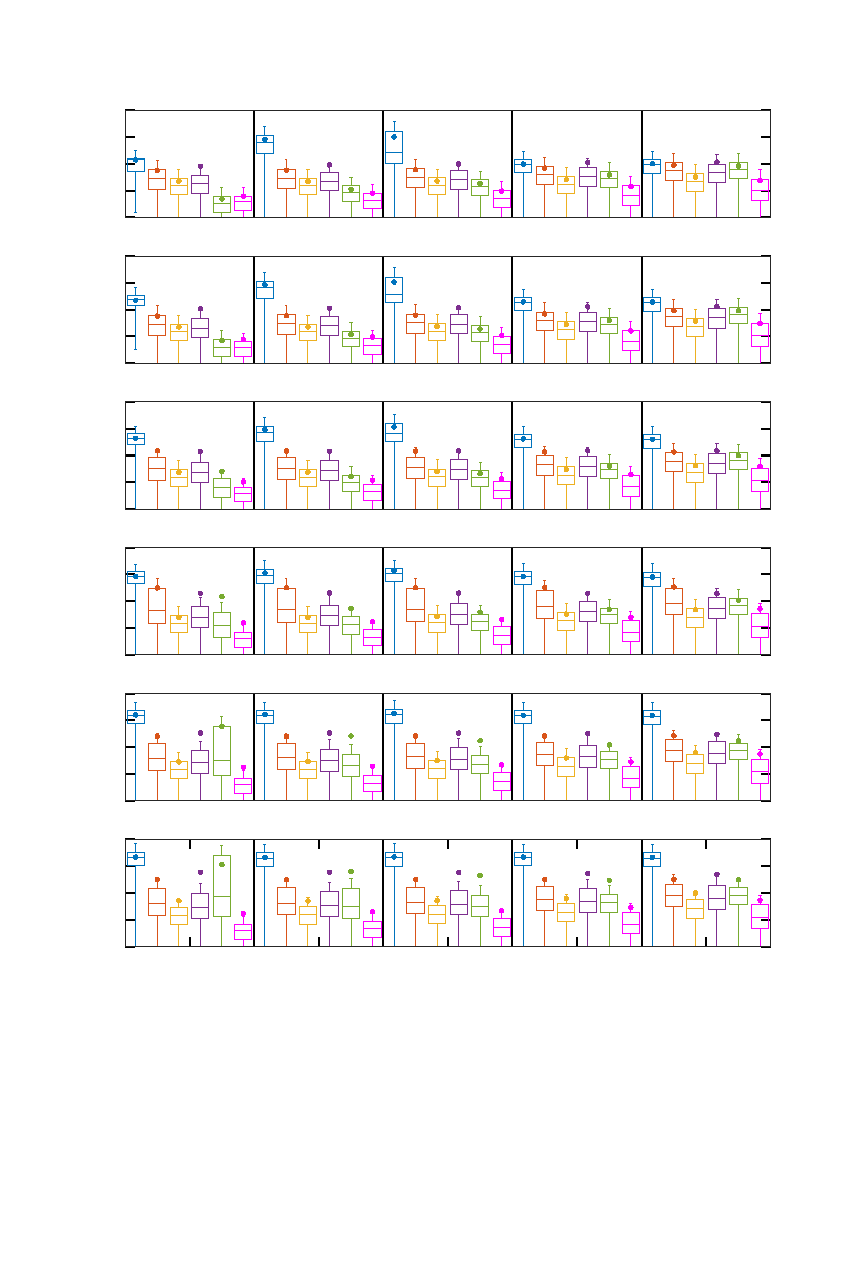
\includegraphics[clip=true,trim={0 500 0 0}]{./figures/slides/ch7/experiments/orientation_errors}}%
    \put(0,5400){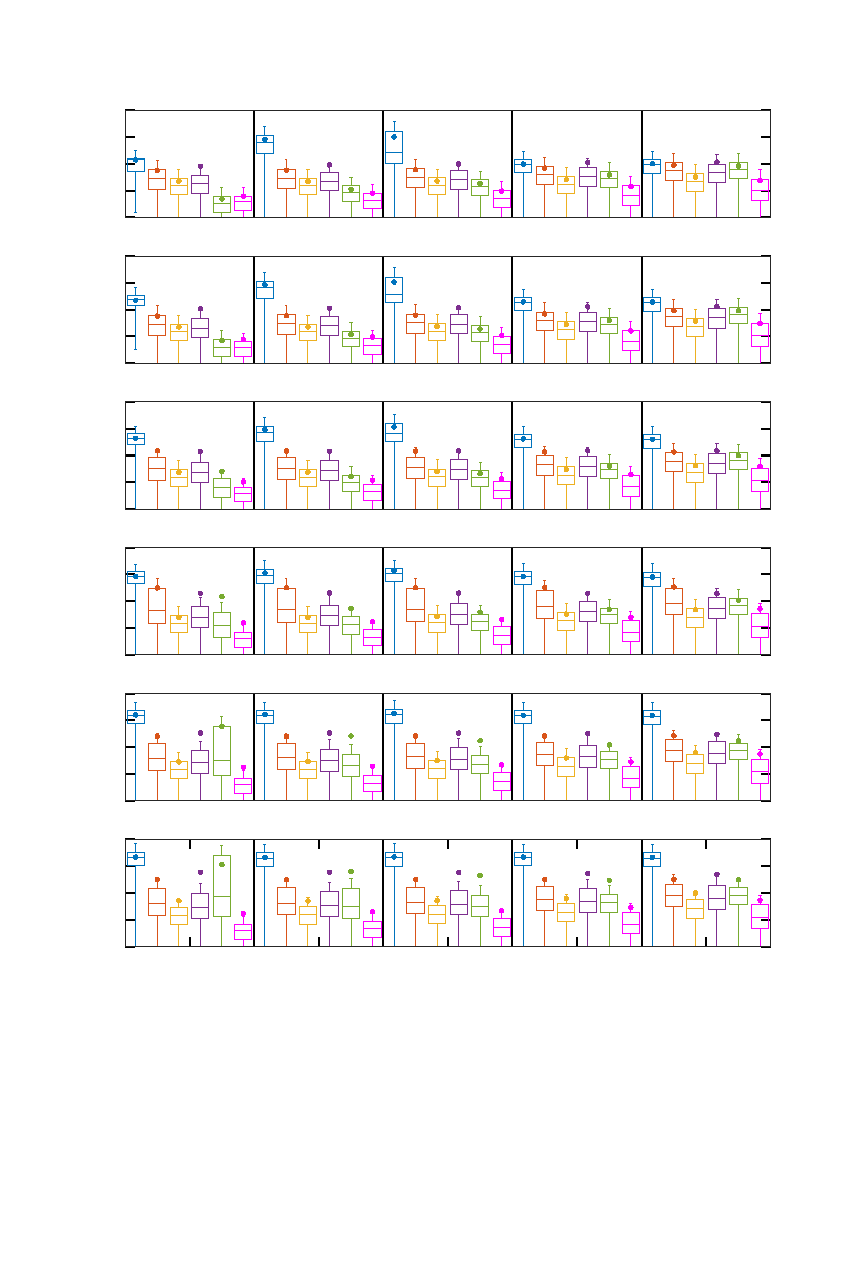
\includegraphics[clip=true,trim = 0 0 0 380]{./figures/slides/ch7/experiments/orientation_errors}}%
    \gplfronttext
  \end{picture}%
\endgroup

  \vspace{-4cm}
  \caption{\small Οι κατανομές των σφαλμάτων εκτίμησης προσανατολισμού για κάθε
           αλγόριθμο με βάση την πειραματική διάταξη της ενότητας
           \ref{subsection:02_05_03:01}. Κάθε ορθογώνιο αντιπροσωπεύει τα
           στατιστικά $\approx 4.5$$\cdot$$10$\texttt{e}$+$$5$ ευθυγραμμίσεων.
           Οι κουκκίδες αντιπροσωπεύουν ολικά μέσα σφάλματα εκτίμησης}
  \label{fig:02_05_03:02:02}
\end{figure}

\begin{figure}\vspace{1cm}\hspace{0.5cm}
  \definecolor{c1}{rgb}{0 0.4470 0.7410}
\definecolor{c2}{rgb}{0.8500 0.3250 0.0980}
\definecolor{c3}{rgb}{0.9290 0.6940 0.1250}
\definecolor{c4}{rgb}{0.4940 0.1840 0.5560}
\definecolor{c5}{rgb}{0.4660 0.6740 0.1880}
\definecolor{c9}{RGB}{255,0,255}

% GNUPLOT: LaTeX picture with Postscript
\begingroup
  \makeatletter
  \providecommand\color[2][]{%
    \GenericError{(gnuplot) \space\space\space\@spaces}{%
      Package color not loaded in conjunction with
      terminal option `colourtext'%
    }{See the gnuplot documentation for explanation.%
    }{Either use 'blacktext' in gnuplot or load the package
      color.sty in LaTeX.}%
    \renewcommand\color[2][]{}%
  }%
  \providecommand\includegraphics[2][]{%
    \GenericError{(gnuplot) \space\space\space\@spaces}{%
      Package graphicx or graphics not loaded%
    }{See the gnuplot documentation for explanation.%
    }{The gnuplot epslatex terminal needs graphicx.sty or graphics.sty.}%
    \renewcommand\includegraphics[2][]{}%
  }%
  \providecommand\rotatebox[2]{#2}%
  \@ifundefined{ifGPcolor}{%
    \newif\ifGPcolor
    \GPcolorfalse
  }{}%
  \@ifundefined{ifGPblacktext}{%
    \newif\ifGPblacktext
    \GPblacktexttrue
  }{}%
  % define a \g@addto@macro without @ in the name:
  \let\gplgaddtomacro\g@addto@macro
  % define empty templates for all commands taking text:
  \gdef\gplfronttext{}%
  \gdef\gplfronttext{}%
  \makeatother
  \ifGPblacktext
    % no textcolor at all
    \def\colorrgb#1{}%
    \def\colorgray#1{}%
  \else
    % gray or color?
    \ifGPcolor
      \def\colorrgb#1{\color[rgb]{#1}}%
      \def\colorgray#1{\color[gray]{#1}}%
      \expandafter\def\csname LTw\endcsname{\color{white}}%
      \expandafter\def\csname LTb\endcsname{\color{black}}%
      \expandafter\def\csname LTa\endcsname{\color{black}}%
      \expandafter\def\csname LT0\endcsname{\color[rgb]{1,0,0}}%
      \expandafter\def\csname LT1\endcsname{\color[rgb]{0,1,0}}%
      \expandafter\def\csname LT2\endcsname{\color[rgb]{0,0,1}}%
      \expandafter\def\csname LT3\endcsname{\color[rgb]{1,0,1}}%
      \expandafter\def\csname LT4\endcsname{\color[rgb]{0,1,1}}%
      \expandafter\def\csname LT5\endcsname{\color[rgb]{1,1,0}}%
      \expandafter\def\csname LT6\endcsname{\color[rgb]{0,0,0}}%
      \expandafter\def\csname LT7\endcsname{\color[rgb]{1,0.3,0}}%
      \expandafter\def\csname LT8\endcsname{\color[rgb]{0.5,0.5,0.5}}%
    \else
      % gray
      \def\colorrgb#1{\color{black}}%
      \def\colorgray#1{\color[gray]{#1}}%
      \expandafter\def\csname LTw\endcsname{\color{white}}%
      \expandafter\def\csname LTb\endcsname{\color{black}}%
      \expandafter\def\csname LTa\endcsname{\color{black}}%
      \expandafter\def\csname LT0\endcsname{\color{black}}%
      \expandafter\def\csname LT1\endcsname{\color{black}}%
      \expandafter\def\csname LT2\endcsname{\color{black}}%
      \expandafter\def\csname LT3\endcsname{\color{black}}%
      \expandafter\def\csname LT4\endcsname{\color{black}}%
      \expandafter\def\csname LT5\endcsname{\color{black}}%
      \expandafter\def\csname LT6\endcsname{\color{black}}%
      \expandafter\def\csname LT7\endcsname{\color{black}}%
      \expandafter\def\csname LT8\endcsname{\color{black}}%
    \fi
  \fi
    \setlength{\unitlength}{0.0500bp}%
    \ifx\gptboxheight\undefined%
      \newlength{\gptboxheight}%
      \newlength{\gptboxwidth}%
      \newsavebox{\gptboxtext}%
    \fi%
    \setlength{\fboxrule}{0.5pt}%
    \setlength{\fboxsep}{1pt}%
\begin{picture}(8000.00,12000.00)%
    \gplgaddtomacro\gplfronttext{%
      \put(4000,12219){\makebox(0,0){\strut{}Κατανομές χρόνων εκτέλεσης [ms]}}%
      \put(1000,11719){\makebox(0,0){\strut{}{\color{c1}{\rule[0.6mm]{0.5cm}{0.5mm}}}\small PLICP}}
      \put(2000,11719){\makebox(0,0){\strut{}{\color{c2}{\rule[0.6mm]{0.5cm}{0.5mm}}}\small NDT}}
      \put(3000,11719){\makebox(0,0){\strut{}{\color{c3}{\rule[0.6mm]{0.5cm}{0.5mm}}}\small FastGICP}}
      \put(4400,11719){\makebox(0,0){\strut{}{\color{c4}{\rule[0.6mm]{0.5cm}{0.5mm}}}\small FastVGICP}}
      \put(5800,11719){\makebox(0,0){\strut{}{\color{c5}{\rule[0.6mm]{0.5cm}{0.5mm}}}\small NDT-PSO}}
      \put(6900,11719){\makebox(0,0){\strut{}{\color{c9}{\rule[0.6mm]{0.5cm}{0.5mm}}}\small \texttt{fsm}}}
      \colorrgb{0.15,0.15,0.15}%
      \put(908,10069){\makebox(0,0)[r]{\strut{}$0.0$}}%
      \colorrgb{0.15,0.15,0.15}%
      \put(908,10799){\makebox(0,0)[r]{\strut{}$50.0$}}%
      \colorrgb{0.15,0.15,0.15}%
      %\put(908,10928){\makebox(0,0)[r]{\strut{}$100$}}%
      %\colorrgb{0.15,0.15,0.15}%
      %\put(908,11004){\makebox(0,0)[r]{\strut{}$150$}}%
      %\colorrgb{0.15,0.15,0.15}%
      %\put(908,11057){\makebox(0,0)[r]{\strut{}$200$}}%
      \colorrgb{0.15,0.15,0.15}%
      \put(908,11099){\makebox(0,0)[r]{\strut{}$250.0$}}%
    }%
    \gplgaddtomacro\gplfronttext{%
      \colorrgb{0.00,0.00,0.00}%
      \put(4139,11219){\makebox(0,0){\strut{}\scriptsize $(\overline{\delta}_{xy}, \overline{\delta}_\theta) = (0.05 \ \text{m}, 0.035 \ \text{rad})$}}%
    }%
    \gplgaddtomacro\gplfronttext{%
      \colorrgb{0.15,0.15,0.15}%
      \put(908,8669){\makebox(0,0)[r]{\strut{}$0.0$}}%
      \colorrgb{0.15,0.15,0.15}%
      \put(908,9399){\makebox(0,0)[r]{\strut{}$50.0$}}%
      \colorrgb{0.15,0.15,0.15}%
      %\put(908,9528){\makebox(0,0)[r]{\strut{}$100$}}%
      %\colorrgb{0.15,0.15,0.15}%
      %\put(908,9604){\makebox(0,0)[r]{\strut{}$150$}}%
      %\colorrgb{0.15,0.15,0.15}%
      %\put(908,9657){\makebox(0,0)[r]{\strut{}$200$}}%
      \colorrgb{0.15,0.15,0.15}%
      \put(908,9699){\makebox(0,0)[r]{\strut{}$250.0$}}%
    }%
    \gplgaddtomacro\gplfronttext{%
      \colorrgb{0.00,0.00,0.00}%
      \put(4139,9819){\makebox(0,0){\strut{}\scriptsize $(\overline{\delta}_{xy}, \overline{\delta}_\theta) = (0.10 \ \text{m}, 0.07 \ \text{rad})$}}%
    }%
    \gplgaddtomacro\gplfronttext{%
      \colorrgb{0.15,0.15,0.15}%
      \put(908,7269){\makebox(0,0)[r]{\strut{}$0.0$}}%
      \colorrgb{0.15,0.15,0.15}%
      \put(908,7999){\makebox(0,0)[r]{\strut{}$50.0$}}%
      \colorrgb{0.15,0.15,0.15}%
      %\put(908,8128){\makebox(0,0)[r]{\strut{}$100$}}%
      %\colorrgb{0.15,0.15,0.15}%
      %\put(908,8204){\makebox(0,0)[r]{\strut{}$150$}}%
      %\colorrgb{0.15,0.15,0.15}%
      %\put(908,8257){\makebox(0,0)[r]{\strut{}$200$}}%
      \colorrgb{0.15,0.15,0.15}%
      \put(908,8299){\makebox(0,0)[r]{\strut{}$250.0$}}%
    }%
    \gplgaddtomacro\gplfronttext{%
      \colorrgb{0.15,0.15,0.15}%
      \colorrgb{0.00,0.00,0.00}%
      \put(4139,8419){\makebox(0,0){\strut{}\scriptsize $(\overline{\delta}_{xy}, \overline{\delta}_\theta) = (0.15 \ \text{m}, 0.15 \ \text{rad})$}}%
    }%
    \gplgaddtomacro\gplfronttext{%
      \colorrgb{0.15,0.15,0.15}%
      \put(908,5869){\makebox(0,0)[r]{\strut{}$0.0$}}%
      \colorrgb{0.15,0.15,0.15}%
      \put(908,6599){\makebox(0,0)[r]{\strut{}$50.0$}}%
      \colorrgb{0.15,0.15,0.15}%
      %\put(908,6728){\makebox(0,0)[r]{\strut{}$100$}}%
      %\colorrgb{0.15,0.15,0.15}%
      %\put(908,6804){\makebox(0,0)[r]{\strut{}$150$}}%
      %\colorrgb{0.15,0.15,0.15}%
      %\put(908,6857){\makebox(0,0)[r]{\strut{}$200$}}%
      \colorrgb{0.15,0.15,0.15}%
      \put(908,6899){\makebox(0,0)[r]{\strut{}$250.0$}}%
    }%
    \gplgaddtomacro\gplfronttext{%
      \colorrgb{0.00,0.00,0.00}%
      \put(4139,7019){\makebox(0,0){\strut{}\scriptsize $(\overline{\delta}_{xy}, \overline{\delta}_\theta) = (0.20 \ \text{m}, 0.30 \ \text{rad})$}}%
    }%
    \gplgaddtomacro\gplfronttext{%
      \colorrgb{0.15,0.15,0.15}%
      \put(908,4469){\makebox(0,0)[r]{\strut{}$0.0$}}%
      \colorrgb{0.15,0.15,0.15}%
      \put(908,5199){\makebox(0,0)[r]{\strut{}$50.0$}}%
      \colorrgb{0.15,0.15,0.15}%
      %\put(908,5328){\makebox(0,0)[r]{\strut{}$100$}}%
      %\colorrgb{0.15,0.15,0.15}%
      %\put(908,5404){\makebox(0,0)[r]{\strut{}$150$}}%
      %\colorrgb{0.15,0.15,0.15}%
      %\put(908,5457){\makebox(0,0)[r]{\strut{}$200$}}%
      \colorrgb{0.15,0.15,0.15}%
      \put(908,5499){\makebox(0,0)[r]{\strut{}$250.0$}}%
    }%
    \gplgaddtomacro\gplfronttext{%
      \colorrgb{0.00,0.00,0.00}%
      \put(4139,5619){\makebox(0,0){\strut{}\scriptsize $(\overline{\delta}_{xy}, \overline{\delta}_\theta) = (0.20 \ \text{m}, 0.56 \ \text{rad})$}}%
    }%
    \gplgaddtomacro\gplfronttext{%
      \colorrgb{0.15,0.15,0.15}%
      \put(908,3069){\makebox(0,0)[r]{\strut{}$0.0$}}%
      \colorrgb{0.15,0.15,0.15}%
      \put(908,3799){\makebox(0,0)[r]{\strut{}$50.0$}}%
      \colorrgb{0.15,0.15,0.15}%
      %\put(908,3928){\makebox(0,0)[r]{\strut{}$100$}}%
      %\colorrgb{0.15,0.15,0.15}%
      %\put(908,4004){\makebox(0,0)[r]{\strut{}$150$}}%
      %\colorrgb{0.15,0.15,0.15}%
      %\put(908,4057){\makebox(0,0)[r]{\strut{}$200$}}%
      \colorrgb{0.15,0.15,0.15}%
      \put(908,4099){\makebox(0,0)[r]{\strut{}$250.0$}}%
      \colorrgb{0.15,0.15,0.15}%
      \put(1660,2849){\makebox(0,0){\strut{}$0.01$}}%
      \colorrgb{0.15,0.15,0.15}%
      \put(2900,2849){\makebox(0,0){\strut{}$0.03$}}%
      \colorrgb{0.15,0.15,0.15}%
      \put(4140,2849){\makebox(0,0){\strut{}$0.05$}}%
      \colorrgb{0.15,0.15,0.15}%
      \put(5379,2849){\makebox(0,0){\strut{}$0.10$}}%
      \colorrgb{0.15,0.15,0.15}%
      \put(6619,2849){\makebox(0,0){\strut{}$0.20$}}%
    }%
    \gplgaddtomacro\gplfronttext{%
      \colorrgb{0.15,0.15,0.15}%
      \put(4139,2519){\makebox(0,0){\strut{}Τυπική απόκλιση διαταραχών $\sigma_R$ [m]}}%
      \colorrgb{0.00,0.00,0.00}%
      \put(4139,4219){\makebox(0,0){\strut{}\scriptsize $(\overline{\delta}_{xy}, \overline{\delta}_\theta) = (0.20 \ \text{m}, \pi/4 \ \text{rad})$}}%
    }%
    \put(0,0){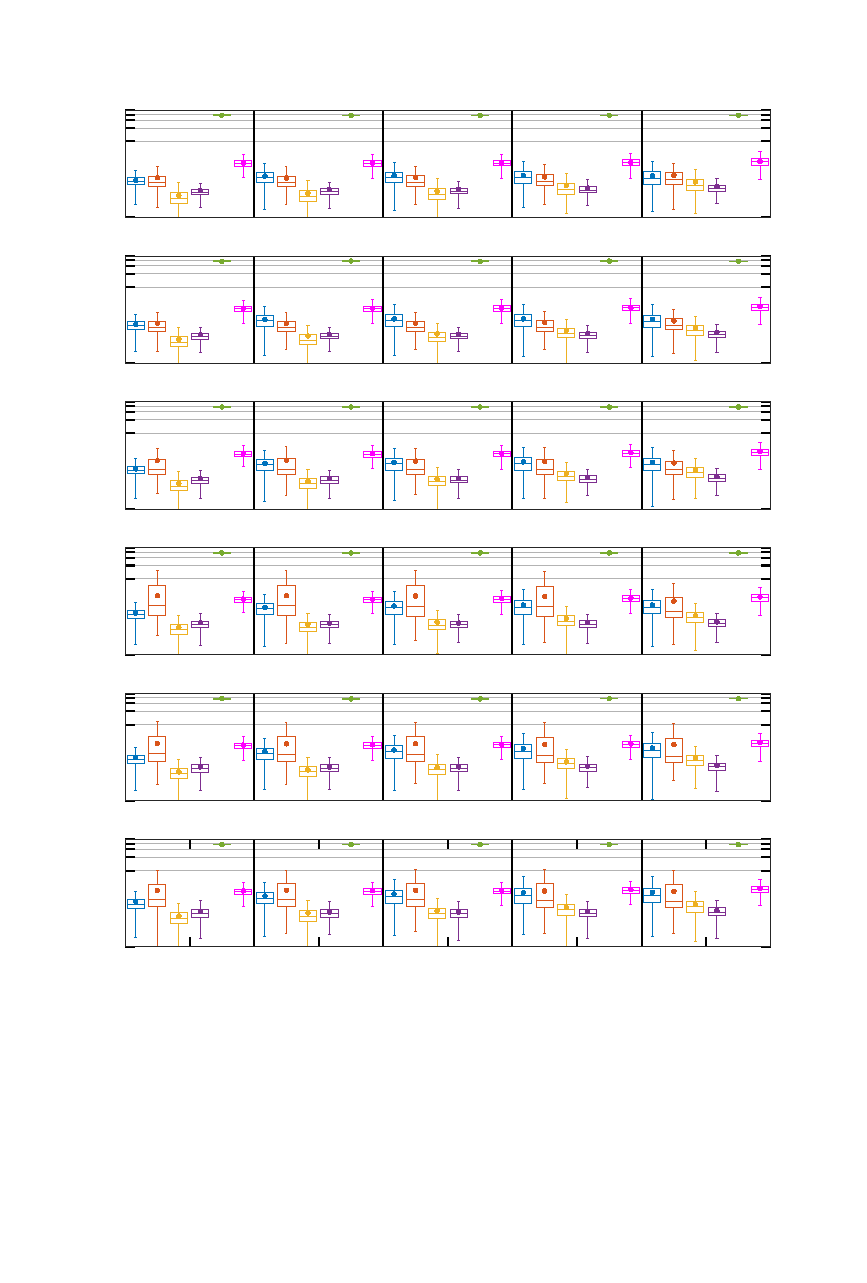
\includegraphics{./figures/parts/02/chapters/05/sections/04/total_times}}%
    \gplfronttext
  \end{picture}%
\endgroup

  \vspace{-4cm}
  \caption{\small Οι κατανομές των χρόνων εκτέλεσης κάθε
           αλγορίθμου με βάση την πειραματική διάταξη της ενότητας
           \ref{subsection:02_05_03:01}. Κάθε ορθογώνιο αντιπροσωπεύει τα
           στατιστικά $\approx 4.5$$\cdot$$10$\texttt{e}$+$$5$ ευθυγραμμίσεων.
           Οι κουκκίδες αντιπροσωπεύουν ολικούς μέσους χρόνους εκτέλεσης}
  \label{fig:02_05_03:02:03}
\end{figure}

\begin{figure}\vspace{1cm}\hspace{0.5cm}
  \input{./figures/parts/02/chapters/05/sections/03/caer_style_position_errors_binned_dxyt6.tex}
  \vspace{1cm}
  \caption{\small Χάρτες θερμότητας των μέτρων των τελικών σφαλμάτων εκτίμησης
           θέσης συναρτήσει των αρχικών σφαλμάτων εκτίμησης προσανατολισμού
           $\Delta\hat{\theta} \in
           [-\overline{\delta}_{\theta},+\overline{\delta}_{\theta}]$ (στον
           οριζόντιο άξονα) και των μέτρων των αρχικών σφαλμάτων εκτίμησης
           θέσης $\|\Delta \hat{\bm{l}}\|_2 \in [0, \sqrt{2}\cdot
           \overline{\delta}_{xy}]$ (στον κάθετο άξονα) για όλα τα
           διενεργηθέντα πειράματα, ανά αλγόριθμο και ανά τυπική απόκλιση
           διαταραχών του φυσικού αισθητήρα, για τη διάταξη με
           $(\overline{\delta}_{xy}, \overline{\delta}_{\theta}) = (0.20,
           \pi/4)$ [m,rad]}
  \label{fig:02_05_03:02:04}
\end{figure}


\begin{figure}\vspace{1cm}\hspace{0.5cm}
  \input{./figures/parts/02/chapters/05/sections/03/caer_style_orientation_errors_binned_dxyt6.tex}
  \vspace{1cm}
  \caption{\small Χάρτες θερμότητας των μέτρων των τελικών σφαλμάτων εκτίμησης
           προσανατολισμού συναρτήσει των αρχικών σφαλμάτων εκτίμησης
           προσανατολισμού $\Delta\hat{\theta} \in
           [-\overline{\delta}_{\theta},+\overline{\delta}_{\theta}]$ (στον
           οριζόντιο άξονα) και των μέτρων των αρχικών σφαλμάτων εκτίμησης
           θέσης $\|\Delta \hat{\bm{l}}\|_2 \in [0, \sqrt{2}\cdot
           \overline{\delta}_{xy}]$ (στον κάθετο άξονα) για όλα τα
           διενεργηθέντα πειράματα, ανά αλγόριθμο και ανά τυπική απόκλιση
           διαταραχών του φυσικού αισθητήρα, για τη διάταξη με
           $(\overline{\delta}_{xy}, \overline{\delta}_{\theta}) = (0.20,
           \pi/4)$ [m,rad]}
  \label{fig:02_05_03:02:05}
\end{figure}


\begin{figure}\vspace{1cm}\hspace{0.5cm}
  \input{./figures/parts/02/chapters/05/sections/03/caer_style_position_errors_dxyt6.tex}
  \vspace{1cm}
  \caption{\small Χάρτες θερμότητας των μέτρων των τελικών σφαλμάτων εκτίμησης
           θέσης συναρτήσει των αρχικών σφαλμάτων εκτίμησης προσανατολισμού
           $\Delta\hat{\theta} \in
           [-\overline{\delta}_{\theta},+\overline{\delta}_{\theta}]$ (στον
           οριζόντιο άξονα) και των μέτρων των αρχικών σφαλμάτων εκτίμησης
           θέσης $\|\Delta \hat{\bm{l}}\|_2 \in [0, \sqrt{2}\cdot
           \overline{\delta}_{xy}]$ (στον κάθετο άξονα) για όλα τα
           διενεργηθέντα πειράματα, ανά αλγόριθμο και ανά τυπική απόκλιση
           διαταραχών του φυσικού αισθητήρα, για τη διάταξη με
           $(\overline{\delta}_{xy}, \overline{\delta}_{\theta}) = (0.20,
           \pi/4)$ [m,rad], εστιασμένοι στο διάστημα $[0,
           e_{xy,\text{avg}}^{\overline{\delta}_{xy},
           \overline{\delta}_{\theta}}]$, όπου με
           $e_{xy,\text{avg}}^{\overline{\delta}_{xy},
           \overline{\delta}_{\theta}}$ σημειώνεται ο μέσος όρος σφάλματος
           εκτίμησης στάσης όλων των μεθόδων, για κάθε επεξεργασθέν δείγμα, και
           κάθε τιμή τυπικής απόκλισης των διαταραχών που επιδρούν στις
           μετρήσεις του φυσικού αισθητήρα, για τη διαμόρφωση
           $(\overline{\delta}_{xy}, \overline{\delta}_{\theta})$.  Τιμές
           μέτρου σφάλματος εκτίμησης άνω του μέσου όρου σημειώνονται με μαύρο
           χρώμα}
  \label{fig:02_05_03:02:06}
\end{figure}


\begin{figure}\vspace{1cm}\hspace{0.5cm}
  \input{./figures/parts/02/chapters/05/sections/03/caer_style_orientation_errors_dxyt6.tex}
  \vspace{1cm}
  \caption{\small Χάρτες θερμότητας των μέτρων των τελικών σφαλμάτων εκτίμησης
           προσανατολισμού συναρτήσει των αρχικών σφαλμάτων εκτίμησης
           προσανατολισμού $\Delta\hat{\theta} \in
           [-\overline{\delta}_{\theta},+\overline{\delta}_{\theta}]$ (στον
           οριζόντιο άξονα) και των μέτρων των αρχικών σφαλμάτων εκτίμησης
           θέσης $\|\Delta \hat{\bm{l}}\|_2 \in [0, \sqrt{2}\cdot
           \overline{\delta}_{xy}]$ (στον κάθετο άξονα) για όλα τα
           διενεργηθέντα πειράματα, ανά αλγόριθμο και ανά τυπική απόκλιση
           διαταραχών του φυσικού αισθητήρα, για τη διάταξη με
           $(\overline{\delta}_{xy}, \overline{\delta}_{\theta}) = (0.20,
           \pi/4)$ [m,rad], εστιασμένοι στο διάστημα $[0,
           e_{xy,\text{avg}}^{\overline{\delta}_{xy},
           \overline{\delta}_{\theta}}]$, όπου με
           $e_{xy,\text{avg}}^{\overline{\delta}_{xy},
           \overline{\delta}_{\theta}}$ σημειώνεται ο μέσος όρος σφάλματος
           εκτίμησης στάσης όλων των μεθόδων, για κάθε επεξεργασθέν δείγμα, και
           κάθε τιμή τυπικής απόκλισης των διαταραχών που επιδρούν στις
           μετρήσεις του φυσικού αισθητήρα, για τη διαμόρφωση
           $(\overline{\delta}_{xy}, \overline{\delta}_{\theta})$.  Τιμές
           μέτρου σφάλματος εκτίμησης άνω του μέσου όρου σημειώνονται με μαύρο
           χρώμα}
  \label{fig:02_05_03:02:07}
\end{figure}

\begin{figure}\vspace{1cm}\hspace{0.5cm}
  \definecolor{c1}{RGB}{3,2,64}
\definecolor{c2}{RGB}{0,0,0}
\definecolor{c3}{RGB}{255,255,251}



% GNUPLOT: LaTeX picture with Postscript
\begingroup
  \makeatletter
  \providecommand\color[2][]{%
    \GenericError{(gnuplot) \space\space\space\@spaces}{%
      Package color not loaded in conjunction with
      terminal option `colourtext'%
    }{See the gnuplot documentation for explanation.%
    }{Either use 'blacktext' in gnuplot or load the package
      color.sty in LaTeX.}%
    \renewcommand\color[2][]{}%
  }%
  \providecommand\includegraphics[2][]{%
    \GenericError{(gnuplot) \space\space\space\@spaces}{%
      Package graphicx or graphics not loaded%
    }{See the gnuplot documentation for explanation.%
    }{The gnuplot epslatex terminal needs graphicx.sty or graphics.sty.}%
    \renewcommand\includegraphics[2][]{}%
  }%
  \providecommand\rotatebox[2]{#2}%
  \@ifundefined{ifGPcolor}{%
    \newif\ifGPcolor
    \GPcolorfalse
  }{}%
  \@ifundefined{ifGPblacktext}{%
    \newif\ifGPblacktext
    \GPblacktexttrue
  }{}%
  % define a \g@addto@macro without @ in the name:
  \let\gplgaddtomacro\g@addto@macro
  % define empty templates for all commands taking text:
  \gdef\gplfronttext{}%
  \gdef\gplfronttext{}%
  \makeatother
  \ifGPblacktext
    % no textcolor at all
    \def\colorrgb#1{}%
    \def\colorgray#1{}%
  \else
    % gray or color?
    \ifGPcolor
      \def\colorrgb#1{\color[rgb]{#1}}%
      \def\colorgray#1{\color[gray]{#1}}%
      \expandafter\def\csname LTw\endcsname{\color{white}}%
      \expandafter\def\csname LTb\endcsname{\color{black}}%
      \expandafter\def\csname LTa\endcsname{\color{black}}%
      \expandafter\def\csname LT0\endcsname{\color[rgb]{1,0,0}}%
      \expandafter\def\csname LT1\endcsname{\color[rgb]{0,1,0}}%
      \expandafter\def\csname LT2\endcsname{\color[rgb]{0,0,1}}%
      \expandafter\def\csname LT3\endcsname{\color[rgb]{1,0,1}}%
      \expandafter\def\csname LT4\endcsname{\color[rgb]{0,1,1}}%
      \expandafter\def\csname LT5\endcsname{\color[rgb]{1,1,0}}%
      \expandafter\def\csname LT6\endcsname{\color[rgb]{0,0,0}}%
      \expandafter\def\csname LT7\endcsname{\color[rgb]{1,0.3,0}}%
      \expandafter\def\csname LT8\endcsname{\color[rgb]{0.5,0.5,0.5}}%
    \else
      % gray
      \def\colorrgb#1{\color{black}}%
      \def\colorgray#1{\color[gray]{#1}}%
      \expandafter\def\csname LTw\endcsname{\color{white}}%
      \expandafter\def\csname LTb\endcsname{\color{black}}%
      \expandafter\def\csname LTa\endcsname{\color{black}}%
      \expandafter\def\csname LT0\endcsname{\color{black}}%
      \expandafter\def\csname LT1\endcsname{\color{black}}%
      \expandafter\def\csname LT2\endcsname{\color{black}}%
      \expandafter\def\csname LT3\endcsname{\color{black}}%
      \expandafter\def\csname LT4\endcsname{\color{black}}%
      \expandafter\def\csname LT5\endcsname{\color{black}}%
      \expandafter\def\csname LT6\endcsname{\color{black}}%
      \expandafter\def\csname LT7\endcsname{\color{black}}%
      \expandafter\def\csname LT8\endcsname{\color{black}}%
    \fi
  \fi
    \setlength{\unitlength}{0.0500bp}%
    \ifx\gptboxheight\undefined%
      \newlength{\gptboxheight}%
      \newlength{\gptboxwidth}%
      \newsavebox{\gptboxtext}%
    \fi%
    \setlength{\fboxrule}{0.5pt}%
    \setlength{\fboxsep}{1pt}%
\begin{picture}(8000.00,10000.00)%
    \gplgaddtomacro\gplfronttext{%
    }%
    \gplgaddtomacro\gplfronttext{%
      \colorrgb{0.15,0.15,0.15}%
      \put(800,8600){\makebox(0,0){\strut{}\small $\sigma_R = 0.01$}}%
      \colorrgb{0.00,0.00,0.00}%
      \put(2400,8600){\makebox(0,0){\strut{}\small $\sigma_R = 0.03$}}%
      \colorrgb{0.00,0.00,0.00}%
      \put(4000,8600){\makebox(0,0){\strut{}\small $\sigma_R = 0.05$}}%
      \colorrgb{0.00,0.00,0.00}%
      \put(5600,8600){\makebox(0,0){\strut{}\small $\sigma_R = 0.10$}}%
      \colorrgb{0.00,0.00,0.00}%
      \put(7200,8600){\makebox(0,0){\strut{}\small $\sigma_R = 0.20$ [m]}}%
      \colorrgb{0.15,0.15,0.15}%
    }%
    \gplgaddtomacro\gplfronttext{%
      \colorrgb{0.15,0.15,0.15}%
      \put(-100,7857.142){\rotatebox{90}{\makebox(0,0){\strut{}\small $\Delta_0$}}}%
      \put(-100,6428.571){\rotatebox{90}{\makebox(0,0){\strut{}\small $\Delta_1$}}}%
      \put(-100,5000)    {\rotatebox{90}{\makebox(0,0){\strut{}\small $\Delta_2$}}}%
      \put(-100,3571.428){\rotatebox{90}{\makebox(0,0){\strut{}\small $\Delta_3$}}}%
      \put(-100,2142.857){\rotatebox{90}{\makebox(0,0){\strut{}\small $\Delta_4$}}}%
      \put(-100,714.285) {\rotatebox{90}{\makebox(0,0){\strut{}\small $\Delta_5$}}}%
    }%

    \gplgaddtomacro\gplfronttext{%
      \put(4000,10100){\makebox(0,0){\strut{}{Αριθμός επανεκκινήσεων ως προς αρχικές συνθήκες}}}
      \put(1333,9520){\makebox(0,0){\strut{}{\color{c1} $0$}}}
      \put(3999,9520){\makebox(0,0){\strut{}{\color{c2} $<10$}}}
      \put(6666,9520){\makebox(0,0){\strut{}{\color{c3} $\leq 100$}}}
    }%

    \put(0,0){
\includegraphics{./figures/parts/02/chapters/05/sections/04/recoveries}}%
    \gplfronttext
  \end{picture}%
\endgroup

  \vspace{1cm}
  \caption{\small Χάρτες θερμότητας του αριθμού των επανεκκινήσεων της μεθόδου
           \texttt{fsm} ανά επίπεδο διαταραχών των μετρήσεων της πραγματικής
           σάρωσης $\sigma_R$ για κάθε διαμόρφωση αρχικών συνθηκών
           $\Delta_\ast$ (Πίνακας \ref{tbl:02:05_03:deltas}), συναρτήσει των
           αρχικών σφαλμάτων εκτίμησης προσανατολισμού $\Delta\hat{\theta} \in
           [-\overline{\delta}_{\theta},+\overline{\delta}_{\theta}]$ (στον
           οριζόντιο άξονα) και των μέτρων των αρχικών σφαλμάτων εκτίμησης
           θέσης $\|\Delta \hat{\bm{l}}\|_2 \in [0, \sqrt{2}\cdot
           \overline{\delta}_{xy}]$ (στον κάθετο άξονα) για όλα τα
           διενεργηθέντα πειράματα}
  \label{fig:02_05_03:02:08}
\end{figure}

%%%%%%%%%%%%%%%%%%%%%%%%%%%%%%%%%%%%%%%%%%%%%%%%%%%%%%%%%%%%%%%%%%%%%%%%%%%%%%%%
\subsection{Εξέταση και αξιολόγηση αποτελεσμάτων}
\label{subsection:02_05_03:03}


